
\clearemptydoublepage
\part{Depiction of the context} % 25p
\label{p:context}


\epigraph{You still don't understand what you're dealing with, do you? The perfect organism. Its structural perfection is matched only by its hostility.}{\emph{Ash, Alien}}

In this part, we present the context of bringing Cloud applications to
the Edge without meddling in their code, the actors involved, and the
difficulties implied.

%
In~\autoref{chap:cloud}, I first depict the existing and well
known part in this problem, the Cloud computing and in more details,
Cloud applications.

%
Then, in~\autoref{chap:edge}, I state what is the new paradigm, Edge
computing and what can be expected from Edge infrastructures.

%
Finally, in~\autoref{chap:cloud-app-to-edge}, I develop an overview
of what is needed for such infrastructures and why the existing
solutions are not appropriate for the requirements presented.




\begin{comment}
* Background - 20p
** Cloud Applications - 10p
*** What is a Cloud Application - 8p
*** Manage Cloud infrastructures - 2p
** What is the Edge - 10p
*** Definition and purpose - 6p
*** What are the challenges - 2p
*** What are the pre-requisites for an application in such a context - 2p
\end{comment}

% \todono{intro}
% We will first depict the actors in this problem, Cloud applications,
% then what we can expect from Edge infrastructures, and finally an
% overview of why the existing solutions do not correspond to what we
% would like.

\chapter{Cloud Applications for beginners} % 10p
\label{chap:cloud}

In this chapter, we will explain how Cloud applications work, on what
type of infrastructure they run, what is their purpose, what are the
underlying assumptions for their proper functioning, and how we can
manage a Cloud infrastructure with a Cloud application.
%
This chapter is intended to be understandable by people with little to
no background in the Cloud.

\section{What is the Cloud?} % 8p
\label{sec:cloud}

Even if you do not know exactly what the Cloud is, you probably at
least already heard about it before, somewhere, and have a vague idea
of its purpose.
%
A lot of the software you can use now propose offers to save your data
somewhere \emph{safer} than your own computer, namely ``\emph{the
Cloud}''.
%
We will now discuss what it is in more details.

\subsection{A short overview of the Cloud}
\label{ssec:cloud-overview}

Cloud computing allows users to use computing resources (\eg
\glspl{server}, network, storage, etc.) on-demand without them having
to manage these resources more than they need.
%
The main goal is to be able to use resources in computing
infrastructures, without the need to actually operate \emph{physical}
resources.
%
This allows consumers (businesses, users, etc.) to avoid the cost,
complexity and lack of flexibility of having to assemble and maintain
these infrastructures.
%
These computing resources are physically located in \glspl{dc} (\acrshort{DC}),
sometimes huge (some of the largest exceed 1M square
feet~\cite{rankeddc}), and pooled together to
be spent by different users, according to their needs.


\autoref{fig:cloudaas} presents an overview of the services available
in the Cloud.
%
Clients, such as web browsers, IoT devices, actual users, access and
use the Cloud, which can be private (for one organization internally
or externally), public (offered over the public internet), hybrid
(composed from a public and a private part) or multiple (from
different Cloud providers), etc.
%
Usually, the standard services models are presented as layers, from
less to more abstracted resources:

\begin{description}

\item Infrastructure as a Service (\acrshort{iaas}) offers low level
  resources such as physical \glspl{server}, networks, Virtual
  Machines (VM), etc. as usable resources for the clients. As such,
  the clients have control over the deployed applications, networks
  resources, etc. on which they will work. Examples of IaaS are
  \href{https://docs.aws.amazon.com/AWSEC2/latest/UserGuide/concepts.html}{Amazon
    EC2}, \href{https://azure.microsoft.com/en-us/}{Microsoft Azure},
  \href{https://cloud.google.com/compute/}{Google Compute Engine
    (GCE)}, \href{https://www.ovhcloud.com/}{OVHcloud}, etc.

\item In Platform as a Service (\acrshort{paas}), the clients are
offered an environment, as a set of applications deployed, that will
allow them to develop, run and manage
applications. \href{https://www.heroku.com/platform}{Heroku}, or
\href{https://aws.amazon.com/lambda/}{Amazon Lambda} are examples of
PaaS.

\item Software as a Service (\acrshort{saas}) offers direct access to
software. More and more desktop applications now have a Cloud version
to be available for users as it would on their computer, but does not
need the underlying requirements for the users points of access (for
example, a user on its computer or smartphone does not need to have a
large CPU, or storage), since the computing (or storage) will be done
in the Cloud. As the most famous examples, we can cite
\href{https://workspace.google.com/}{Google Workspace},
\href{https://www.microsoft.com/en/microsoft-365/free-office-online-for-the-web}{Microsoft
Office on the web} or \href{https://www.netflix.com}{Netflix}.
\end{description}
%

\begin{figure}[htbp]
  \centering
  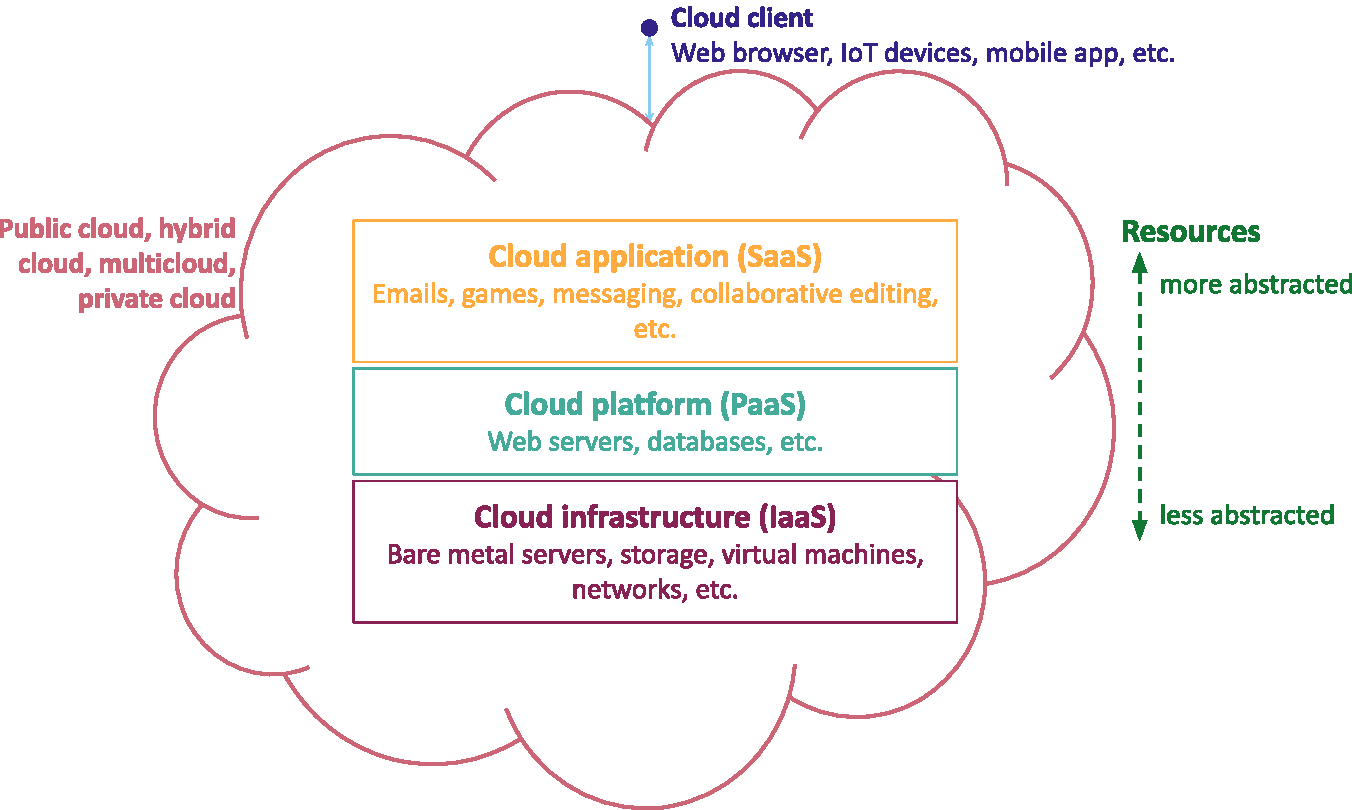
\includegraphics[width=.8\linewidth]{figs/pdf/CloudaaS}
  \caption{Different service models of the Cloud}
  \label{fig:cloudaas}
\end{figure}



To be more formal, the NIST (National Institute of Standards and
Technology) defined 5 principal characteristics for the Cloud
computing model~\cite{MG+11}:
\begin{description}
\item [On-demand self-service.] A user can interact with service
  providers without the need for a human, to get computing resources,
  such as storage, \glspl{server}, network. We will talk more about these
  resources in the next~\autoref{ssec:cloud-infra}.
\item [Broad network access.] These resources are delivered through
  the Internet network and can be accessed from heterogeneous devices
  (mobile phone, laptop, etc.).
\item [Resource pooling.] Cloud computing resources are pooled to
  serve multiple users at the same time (this is called multi-tenancy),
  and can be dynamically assigned depending on demand. Usually, the
  users have neither control nor knowledge of the exact location of
  the resources they are served. Sometimes, they may be able to
  specify the global location (such as country, region, \gls{dc}).
\item [Rapid elasticity.] Resources can be dynamically provisioned,
  used and released to scale up or down automatically per user
  demand. They often can appear virtually unlimited to the users.
\item [Measured service.] The resources usage is monitored, which
  allows to optimize it. This usage can be measured, controlled and
  described to provide transparency for both the users and the provider.
\end{description}


% A really important takeout from this overview of the Cloud is that
% resources managed by applications \emph{of} the Cloud are really
% diverse, from VMs to IPs, from email to text.


\subsection{Cloud Infrastructures}
\label{ssec:cloud-infra}

% To dive more into what a Cloud application is, we have to understand
% what are the characteristics of datacenters.

Whether we are speaking of large \dcs or smaller, on premises, sets of
hardware components, Cloud infrastructures building blocks are usually
collocated and as homogeneous as possible. This is the hardware layer.

An abstraction layer virtualizing resources is often used to bring a
better infrastructure logic to allow network and system administrators
to manage these infrastructures more easily. This is the
infrastructure layer that can be directly offered as a service (IaaS,
as seen in~\autoref{ssec:cloud-overview}). Then come platform and
applications layers (PaaS and SaaS).

Hardware, storage, network and virtualization compose the Cloud
infrastructure.
\begin{description}
\item[Hardware] includes \glspl{server}, as can one expect, but also
  \gls{disk array}s, network components such as \glspl{router},
  \gls{switch}es, etc.
\item[Virtualization] is the component that links physical hardware
  from abstracted layers. Typically, a \gls{hypervisor} abstracts the
  underlying hardware resources to link them logically and make them
  more easy to manage as pools of global resources in the
  infrastructure.
\item[Storage] is managed to back up data automatically or manually,
  ensure that older backups are automatically removed when they are no
  longer relevant, etc. It abstracts the physical storage through
  virtualization to offer Cloud storage solutions.
\item[Network] is composed of the physical network components on which
  virtual networks are created. Typically, virtual networks have
  different virtual resources that can be used, such as static/dynamic
  IPs, private or public sub-networks.
\end{description}

All the virtualized resources, including the network resources, are
pooled as usable entities ``independently'' of the physical resources
under, which means a user can exploit for example storage from two
different parts of the same \dc without even realizing it, as it was
one single entity.



\section{Cloud applications}
\label{sec:cloud-app}

Cloud applications, also called Cloud-native applications because they
were developed specifically for the Cloud, are the software that users
can access to execute services remotely, in \emph{the Cloud}.
%
More specifically, these applications run on top of two systems:
client-side (for example, the users' computer, or their browser) and
server-side (which is contacted by the application on the
client-side).


There are a lot of types of Cloud applications. But for most of them,
they are a set of independent, \gls{loosely coupled}, small \glspl{service},
connected with each other to form an entire, functional application.

In the rest of this thesis manuscript, we will use indiscriminately
\gls{microservice}~\cite{Tho15} or service to define these services
that are used to decouple functionalities in Cloud applications.
%
It is important to define also here that though we talked about
infrastructure computing resources before, from now on, we will use
the word \emph{resource} alone (unless it is obvious we talk about
infrastructure resources) to describe values that can be manipulated
by an application, and some can be stored in a data store, but it is
not mandatory. These resources can also have side effects when
manipulated.


\begin{figure}[htbp]
  \centering
  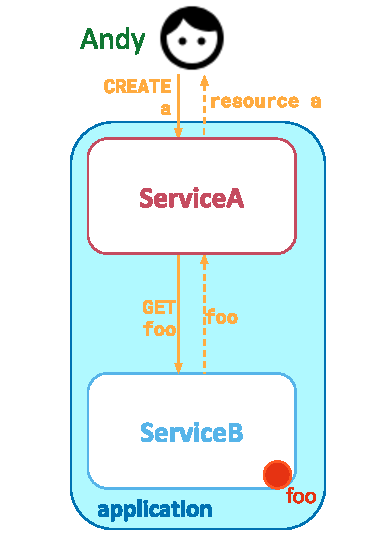
\includegraphics[width=0.3\textwidth]{figs/pdf/application}
  \caption{A typical Cloud application}
  \label{fig:typical-app}
\end{figure}

\autoref{fig:typical-app} presents a typical \gls{microservice} based Cloud
application.
%
The blue rectangle around represents the entire Cloud application.
%
A user (Andy), asks to \verb|CREATE| a resource \verb|a|.
%
The calls are shown in \textbf{{\color{CbOrange}orange}}, full arrows
; the responses in \textbf{{\color{CbOrange}orange}}, dashed
arrows.
%
\textbf{{\color{CbRose}ServiceA}} represents the service called by
Andy, which requires a sub-resource \verb|foo| from
\textbf{{\color{CbCyan}ServiceB}}, to create the requested resource
$a$.
%
Notice that \verb|ServiceA| effectively requests (\verb|GET|)
automatically, by itself, the sub-resource \verb|foo| from
\verb|ServiceB|, without any more intervention from the user.

In a more practical example for this figure, imagine that Andy wants
to create an account on an e-commerce website.
%
\verb|ServiceA| could be the service which creates and manages
accounts, and \verb|ServiceB| a service which creates and manages a
randomly generated image as an avatar for the account.
%
Andy asks an account creation, and \verb|ServiceA| will execute this request,
getting a random image from \verb|ServiceB| to create the account.
%
In this case, resource \verb|a| would consist in different information on
the account, and \verb|foo| the image.


% \todofig{Cloud application with a user using tikz}

% \begin{figure}[htbp]
%     \centering
%     \scalebox{.9}{%
%     \begin{tikzpicture}
%       \node[labeled] (App) {$App$};
%       \service[right=of App.north, matrix anchor=north west]{s}{e,f}
%       \service[right=of s]{t}{g,h}

%       % Workflow
%       \draw [->] (s-2-1) -- (t-3-1);

%       \node (c) [left=12mm of s-2-1] {$\bullet$};
%       \draw [->] (c)      edge (s-2-1.west);
%     \end{tikzpicture}
%     }
%     \caption{Application $App$ made of two services $s$ and $t$ and
%       four endpoints $e, f, g, h$. The $s.e \rightarrow t.h$
%       represents an example of a workflow.}
%     \label{fig:application}
%   \caption{Microservices architecture of a Cloud application}
%   \label{fig:soa}
% \end{figure}



% \section{Manage Cloud infrastructures} % 2p
% \label{sec:cloud-infra}

\section{Conclusion on the Cloud}
\label{sec:cccloud}

The Cloud is composed of hardware and software capabilities offered to
users, who do not have to manage the underlying infrastructure or even
have the compute capabilities.
%
Users only require a device to connect to \emph{the Cloud} thanks to
the device they do have to get the resources they need to complete
their tasks.

%
This comes with benefits such as scalability and flexibility of Cloud
resources, availability of the offered services without having to own
and maintain the required hardware.
%
The Cloud is usually physically located in public or private data
centers, that can be really huge and are typically not really close to
the users, but rather placed where costs for the infrastructure are low.

Cloud applications, running in the Cloud, are the ones that will be
manipulated by users to achieve their goals in the Cloud, and are
often composed of services that fulfill one functionality of the
application and are connected together to achieve the entire
application purpose.

We will now discuss what is the Edge computing paradigm, which comes
from the Cloud computing one.


\chapter{What is the Edge?} % 10p
\label{chap:edge}

In this Chapter, we are going to see what is the Edge and how it
differs from the Cloud.
%
Then, we will discuss what are the challenges of running an
application at the Edge, shedding more light on why it is difficult.

\section{Definition and purpose} % 6p
\label{sec:edge-def}

\subsection{Overview of the Edge}

The Edge is more recent and consisted originally in \glspl{Contentdn}
(\acrshort{CDN}), which \gls{cache}d and delivered large web content
such as videos~\cite{DPW04}. Since then, the technology evolved to deliver more than
static content~\cite{NSS10}.


The best way to envision the Edge as we consider it is to bring the
Cloud (computation and storage) closer to the users.
%
There are a lot of different views on what is the Edge, and how to
define it.%

%
Sometimes called Fog Computing, the part we are interested in is
located in between the Cloud \dcs and small devices that will collect
data or just need some computation to be done~\cite{SPDSM21}.
%
Some people only refer to the Edge as the devices that comprises the
closest devices from the users, and Fog for the layer between this
Edge and the Cloud~\cite{WVMN17}, or Fog as the continuum between Edge
and Cloud~\cite{MWTDV19}, or they use \glspl{cloudlet} as
Fog~\cite{SBCD09}.
%
We refer to those as Edge devices (or sensors and controllers), and
the \glspl{server} were the computation will mostly take place as Edge
\glspl{server}, or Edge \glspl{dc}, or for one set of collocated
\glspl{server}, as an Edge site.
%
Whatever the name, the \emph{Edge \glspl{dc}} will be the ones to
make the hard work, considering the devices at the Edge of the network
won't be able to carry it out, and will only collect data, sometimes
pre-process them\cite{SGDR21, TSS21, WFGI+19}, and in some case, even
those Edge sites will only do some parts, and the bulk of the tasks
will be executed in the Cloud.
%
% In some particular cases such as collaborative (or coordinated)
% applications where users collaborate for some tasks, such as
% \href{https://workspace.google.com/}{Google Doc}, the bulk of the workload will still be done on Edge devices


\begin{figure}
  \centering
  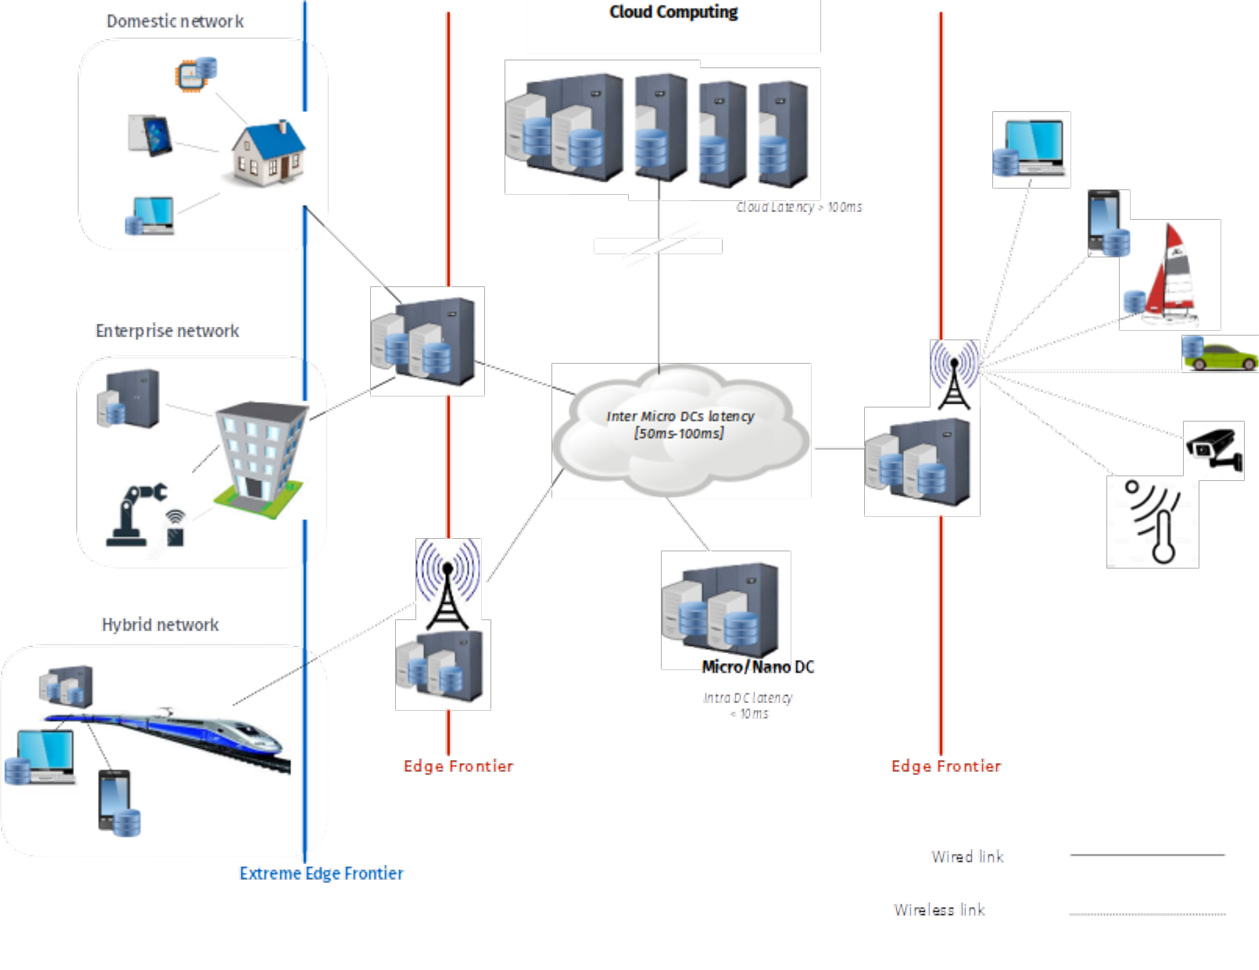
\includegraphics[width=0.8\textwidth]{figs/pdf/edge-infra}
  \caption{An overview of the Cloud and Edge (Source: \href{https://www.usenix.org/sites/default/files/conference/protected-files/hotedge18_slides_cherrueau.pdf}{Usenix - HotEdge'18})}
  \label{fig:edge-infra}
\end{figure}


The \emph{Edge \glspl{dc}} we are considering are thus in charge of
delivering Cloud capabilities to an Edge location (\ie a region, a
city, an business, an airport, etc.) and are composed of up to one
hundred \glspl{server}~\cite{CDL21}.
%
\autoref{fig:edge-infra} presents a view of Cloud \dcs and our
micro/nano-\dcs we discuss about.
%
They can be located anywhere, near the Edge devices, or in
\acrshort{PoP}s, on the Edge frontier.
%
We consider that the latency from clients to the Edge \dcs should be
around or less than 10ms, when the one to Cloud \dcs is between 50 to
100ms (or even more in worse cases, such as 150ms from Paris to Los
Angeles~\cite{pings}).

It is really important to understand that Cloud and Edge are
fundamentally the same in terms of the logic of offering resources,
storage, computing capabilities.
%
One way to see it is: imagine a really small \gls{dc}, and there
are thousands of them, distributed all around the globe.
%



\subsection{Intent}

The most obvious purpose of Edge computing is to improve (lower) the
latency between the location where a request is made and the place
where it is executed.
%
Indeed, since the distance is shorter between them, it is expected
that the response time will improve, on condition that the request is
executed as quickly on an Edge location as it will be further away in
the Cloud.

%
But by executing requests closer to the users, it is also expected to
save a lot of bandwidth on the parts of the network between \emph{the
  Cloud} (Cloud infrastructures) and the Edge.
%
This implies a reduction in data transfer costs.


%
Another potential benefit is to try and use renewable energy to run
the Edge infrastructures, by using farther sites when the closest
location energy is not sufficient to cover the execution of
requests~\cite{LYDP+18}, therefore increasing the sustainability of
the Edge computing~\cite{VLDH+21}.


To explicit the aim of the Edge computing, it is better to state some
of its potential applications.
%
As mentioned, the main purpose of the Edge is to reduce the response
time of \emph{Cloud requests} and execute the requests closer to where
they were made.
%
The Internet of Things (\acrshort{IoT}) is the most common example, with
the need for scalability, and avoiding flooding the usual network with
a lot of data.

\begin{figure}
  \centering
  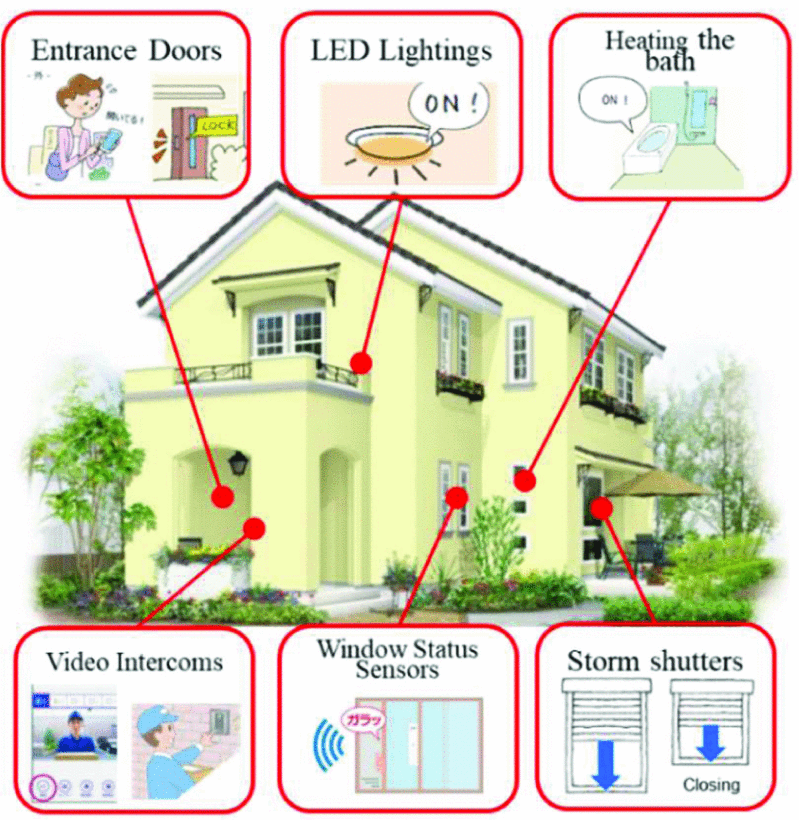
\includegraphics[width=0.6\textwidth]{figs/png/smart-homes}
  \caption{Overview of The Smart Homes from~\cite{II20}© 2020 IEEE}
  \label{fig:smart-home}
\end{figure}

And in particular, to give more concrete examples, Edge computing can
be used, among other use cases, in agriculture, \eg to improve
yield~\cite{SKPJ+19, DC19, JGE17}; in the oil industry, \eg to monitor
the transportation of the oil, for example~\cite{ALSL21, AONOA21}, in
a house, \eg to improve daily life or reduce energy costs~\cite{VBT16,
SH20, II20} or for smart cities~\cite{SKH18, YXCW+15}.
%
\autoref{fig:smart-home} shows examples on how to improve daily life
with smart homes, such as to control via application or automatically
through sensors different appliances in a house.





\section{Hostility of the Edge} % 2p
\label{sec:edge-chal}


% \section{What are the requirements for an application in such a context} % 2p
% \label{sec:edge-req}


Though the Edge can be really powerful to avoid use of bandwidth (by
going more local) and gives a lower latency for the applications
requiring it, there are also some challenges that come with it.

It is a hostile and challenging environment~\cite{MZCBT22, VWBKN16}
for Cloud applications, with \textbf{latency} that come through the
roof when different locations on opposite sides of the globe need to
communicate with each other: the user is indeed closer to one Edge
location, but maybe its request demands a resource that is far away
and will need to be fetched.
%
Moreover, overload can be generated on the network or in the
overall application because of the scale and stability of the system
can highly increase response time~\cite{platform9-latency, SCZKX16}.


Another challenge to be considered is the \textbf{heterogeneity} of
resources on which the applications will run~\cite{HoBl19}.
%
In our case, we do not really consider the Edge devices (\eg
\acrshort{IoT}), but even with small \dcs around the globe, it
implies that probably different actors will be involved.
%
And with different actors, or even often when we consider a single
actor, the infrastructure (hardware, protocols and Operating Systems)
of each site will probably differ from another~\cite{XJLC+19, SCZKX16}.

The \textbf{scale} of the infrastructure is also another
challenge~\cite{edge-challenges, mirantis-edge-challenges}.
%
Having small \glspl{dc} around the globe close to the user
implicitly says that there are going to be a lot of them; and that
the applications running on it need to be highly scalable.


Alongside the two last challenges comes the difficulties of control
and management of those sites, or put differently, the
\textbf{operational constraints}~\cite{edge-challenges, SCZKX16}.
%
First, how to ensure the reliance of the equipment, network, and more
generally the infrastructure environment in such a geo-distributed and
at high scale.
%
Second, how to have a global view of the entire infrastructure
made from so much a large number of site and heterogeneous hardware.
%
And third, how to ensure the security on this infrastructure,
especially how to isolate workload while having a global view.


%
But probably the worst aspect of Edge computing is that
\textbf{disconnections} between Edge locations are the norm rather
than the exception~\cite{SR21, IRPCM22}.
%
This is a huge problem when considering pushing Cloud applications to
the Edge.
%
Cloud applications assume a high reliance of the
infrastructure~\cite{Tamiru21}, so having parts of the pooled
resources from the Edge infrastructure unavailable suddenly is
definitely an issue~\cite{JS20}.

\section{Conclusion on the Edge} % 2p
\label{sec:ccedge}

The Edge computing paradigm has been created to deal with more and
more devices and applications requiring a low latency for the request
they were making to the Cloud.

As several different definitions exist for the Edge, I need to
reiterate here that in this manuscript, we refer as Edge, small
\glspl{dc} (up to a hundred servers), located near the users (less or
around than 10ms latency), that will serve either as the main point of
request executions, or as a relay for small requests, and redirect the
larger requests to the Cloud.

There are a lot of applications for the Edge, but it comes with some
inherent problems to tackle, such as heterogeneity, scale,
operational constraints, and most important, \textbf{frequent
disconnections} and the \textbf{latency} between different sites.

With these specifics in mind, we will now take an interest in how to
put Cloud applications at the Edge.


\chapter{Bringing Cloud applications to the Edge} % 5p
\label{chap:cloud-app-to-edge}



In this chapter, we state the principles and requirements identified
in this thesis as necessary to bring existing Cloud applications to
the Edge considering the challenges mentioned in the previous chapter.


% \section{Which type of Cloud Applications are we talking about}
% \label{sec:app-def}

% why
The main point of this thesis is about bringing existing, functioning
Cloud Applications to the Edge.
%
Since some of these applications are huge, to push these applications
from Cloud to Edge, we want to avoid changing their code as much as
possible.
%
%
These applications had some assumptions about the underlying
infrastructure it would be deployed upon.
%
These assumptions no longer make sense in the Edge context, with
failures and disconnections happening regularly all over the
infrastructure, as was just mentioned in the previous chapter.




\section{Defining principles and expectations}
\label{sec:principles}


In order to deal with the specific challenges stated
in~\autoref{sec:edge-chal}, applications in Edge computing have to
manage the geo-distribution of resources themselves~\cite{TBRT19}.


In~\cite{ST17}, the authors describe a distributed system as:
\begin{quote}
  A distributed system is a collection of autonomous computing
  elements that appears to its users as a single coherent system.
\end{quote}

In a geographically distributed environment, we need to follow two
major principles we introduced in~\cite{CDL21}:

\begin{description}
\item [Local-first]:~Minimize communications between sites and be able
to deal with network partitioning issues by continuing to serve local
requests at least.
 \item [Collaborative-then]:~Be able to take advantage of the
 different sites according to users' needs and infrastructure
 considerations.
\end{description}

The local-first principle has also been defined for \emph{local-first
software} in~\cite{local-first}; with seven ideals that should come
with it: fast, multi-device, ability to function offline,
collaboration between users, longevity, privacy, and user ownership
and control.
%
Moreover, for some applications such as social applications, the
propagation of the content is often localized, so a lot of processing
can be executed close to the point of origin~\cite{WLSY12}.

%
A lot of Cloud applications were created not as monoliths, but by
separating the code into collections of functionalities that apply one
resource or a small set of resources, called services~\cite{JPM+18,
Fie00}, as mentioned in~\autoref{sec:cloud-app}.
%
Some approaches to use Cloud applications at the Edge use this to
deploy different services/functionalities on different sites, or
different instances of the same service on different \glspl{server} or
sites, for balancing purposes~\cite{WVMN17,ROCW14,FLR16} .

From my point of view, the easiest way to ensure the local-first
principle is by having an entire instance of the application on each
site, which coincides with the description of distributed systems
above (autonomous computing elements).
%
%
But autonomous instances alone do not provide a way to ensure the
\emph{collaborative-then} principle.
%
In order to share diverse resources and enhance the capabilities of
the geo-distributed cloud application, an instance on one site should
be able to collaborate with other instances on other sites if need
be~\cite{BJ13}.

With the collaborations between all the instances of every sites, we
can get a single coherent system.
%
This view of a single coherent system I am aiming at and described in
the definition of a distributed system, is also comparable to the
Single System Image (SSI), which is composed of physical or logical
mechanisms to give the illusion that a set of distributed,
heterogeneous resources (hardware) forms a unique and shared computing
resource~\cite{BCJ01}.

With those principles, we can have a geo-distributed application
running at the Edge.
%
But these principles are not enough to specifically bring Cloud
applications to the Edge, with its inherent constraints.
%
Thus, several requirements I deem necessary in this context of
bringing Cloud applications to the Edge follow, with some of them
joining the local-first software ideals.


\begin{description}
\item [Non-intrusive:] One thing we do not want to do is change the
code of the application to geo-distribute it.
%
This is not mandatory for the Edge, but since it is a gain in time, it
is one of the roots of my approach.
%
The main reason is that some Cloud applications are huge and thus
changing their code is tedious and afterwards difficult to maintain.
\item [Generic:] This is not a requirement for the Edge per-say, but
  in order to be largely used, the bulk of the effort to push an
  existing application to the Edge should be (almost) ready to be used
  by developers for their applications, with a minimum production from
  their parts to plug to the solution if necessary.
\item [Tolerance to network partition:] This is the criteria of being
robust to network partition.
%
Since the Edge infrastructure is globally distributed, an application
deployed at the Edge must reckon with the challenges coming with a
wide-area network~\cite{LCR17}, one of them being frequent
disconnections and network partition.
%
It is different from the local-first principle because this is not the
only way to envision tolerance to network partition, such as
replication and distribution of services.
\item [Dynamic placement of requests execution:] The location of
requests execution should be handled dynamically.
%and as much as possible, not statically in a configuration file.
%
In the context of the Edge, it is important that requests can be
executed dynamically as the Edge itself is pretty
dynamic~\cite{FYWCS22}, with nodes connecting and disconnecting often.
%
By default, a static service composition establishes the collaboration
between services inside one instance permanently~\cite{DS05}.
%
It presents great advantages for the developer.
%
Modularity and static composition anticipates the services interface,
behavior and location.
%
Therefore, it guarantees the correctness of services’ invocations and
proper execution of the application~\cite{CJ01}.
%

In \os, for instance, the compute service is configured, once and for
all, to always request the image service in the same DC.
%
Hence, the compute does not mess with an unacquainted service.
%
However, these guarantees comes with the cost of an unyielding
application~\cite{DS05,FS04} that prevents on-the-fly collaborations.
\item [On-demand execution location:] The
location of execution of requests should be chosen per request by the
users of the application for several reasons~\cite{TPTE21}.
%

First, the need for privacy and trust is really important in the
context of the Cloud, and equally important in the Edge.
%
To ensure that the users privacy is respected, it is always easier to
let them choose where their resources will be located and manipulated,
which sites they trust.
%

Second, to avoid overloading each node with resources, it is
appropriate to have public resources scattered across the
infrastructure and usable at will, only when needed.
%
In this regard, it is intimately linked to the collaborative-then
principle.
%

This requirement is crucial, because it is always possible to add a
layer on top that would choose the location of requests execution
either by learning where the users usually execute their requests or
depending on nodes availability and/or latency, or using the
information on the nodes uptime for reliability~\cite{FMPS10, Lim21}.
%
This layer could be added if the need arose to avoid lengthy and
redundant information in requests or if a more transparent definition
is required, \eg for simplicity.
%
But it would be more difficult to give the users the choice of
defining their needs finely, on-demand, rather than automatize everything
from the beginning.
\item [Decentralized:] In the goal of coping with the network faults,
a centralized approach means some of the logic of the application will
not be able to be executed in case of a disconnection (it is a Single
Point of Failure).
%

A centralized approach is also a bottleneck, as all requests that need
to be handled by a central authority will need to go through the same
site, and goes against the goal of lowered latency of the Edge, as
requests will need to go further most of the time (breaking our
local-first principle as well).
\item [\Gls{p2p} (\acrshort{P2P}):] This properties derives from other
aforementioned requirements (local-first, tolerance to network
partitions, decentralized), but adds the necessity for equally
privileged instances of the applications; and it goes along by default
with having autonomous instances of an application everywhere.
%
Moreover, as the main challenges of the Edge are frequent
disconnections, latency and distributed resources between nodes of the
infrastructure, it makes sense to check if the adopted solution can be
considered as \acrshort{P2P} approach as these are the challenges that a
\gls{p2p} system deals with automatically~\cite{Sch01}.
\end{description}




\section{Premises of solutions} % 3p
\label{sec:c-to-e-solutions}



While the local-first principle can be ensured single-handedly by
having an entire instance of an application on each site, it
automatically prevents the use of resources between the sites if the
application was not designed for this.
%

Thus, with such a deployment, we have isolated applications that only
work with their own resources and we do not leverage the overall Edge
infrastructure.
%
Moreover, sharing resources between those different instances makes
sense in the context of the Edge, where the mobility of the users and
the locality of execution is crucial~\cite{SCZKX16, CLPW+18}.
%
Accessing a resource that is on another instance of the application
requires additional pieces of code that is not really dedicated to the
application business, and worse, that only has this particular
function.
%
% Moreover, the challenges of data management in distributed systems
% alone are good reasons to keep this need separated from the
% rest~\cite{Bloom}.

A way to share resources between multiple instances of an application
is to leverage both the service composition and the fact that multiple
instances of an application share the same services, that thus expose
the same \gls{api} (\acrshort{API}).
%
This is simple inter-service communication (ISC) that goes from one
site to another, as it can be used for load-balancing purposes.
%
Unfortunately, though this type of collaboration is easy to realize,
it does not provide a global view that would be expected as one
single, coherent system.

To achieve this view, such as a SSI we mentioned in the
previous~\autoref{sec:principles}, we need to be able to manage
resources between different instances of the same service.
%
To allow this, each service must be extended with some code that
allows more collaboration.
%
We refer to this type of collaboration as intra-service collaboration,
because it is used within the logic of one service, between multiple
instances of the same service.
%
The problem that goes with this dedicated code is that it goes beyond
the initial purpose of the service and thus includes collaboration
code in the business code of the service.
%
Although this dedicated means can benefit from message passing
middlewares or distributed databases internally, it always requires
invasive and complex code~\cite{CDLR+20}.
%
This is a well-known, challenging, and error-prone task for developers
of the application~\cite{ACHM11, BHJL+87, HR85}, who prefer not to
take resource sharing into account most of the time.
%
But the other side is that these sorts of collaborations allow a
global vision of resources managed by the applications, because
users are thus be able to retrieve any resource from anywhere in the
system/infrastructure.


\begin{figure}[htbp]
  \centering
  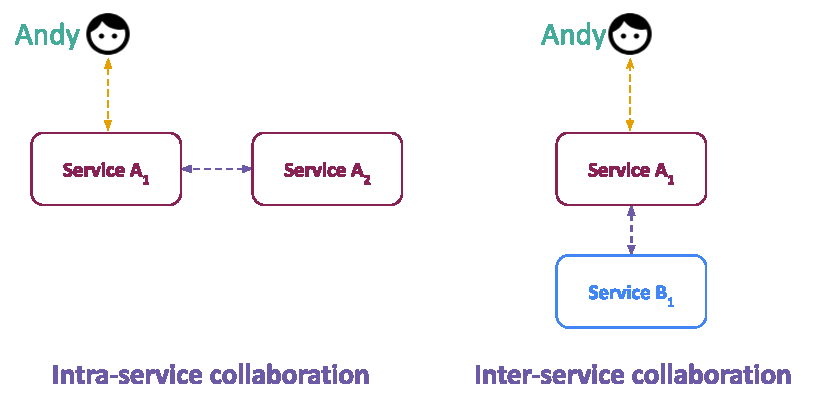
\includegraphics[width=0.8\textwidth]{figs/pdf/collaborations}
  \caption{Intra and inter-service collaborations}
  \label{fig:intera-collabs}
\end{figure}

So we have two types of collaborations between services: intra and
inter.
%
The former implements the collaborations of different instances
of the same service; the latter the collaborations between different
services and, in our case, especially from different services across
application instances or sites.
%
Both types of collaborations are presented
in~\autoref{fig:intera-collabs}.
%
In \textbf{intra-service collaborations}, we can see that the user interacts
with one service, and there is \emph{some kind} of collaboration
between the two instances of the same service to fulfill the request.
%
For example, getting some information from whichever database the
other instance of the service is connected to (assuming they are not
connected to the same database, as they would on two different
autonomous sites).
%
In \textbf{inter-service collaborations}, the
collaboration is made between two different services.
%
In two different instances of an application, it could be possible to
execute this collaboration between two different instances of two
different services.
% such as the case of having one entire application deployed on each
% site,   .
%
Both those types of collaborations ensure a single coherent
system that leverages the entire infrastructure and every resources
available.
%


\section{Why current solutions do not fit all our expectations} % 2p
\label{sec:why-no}

% In the previous section, we discussed how to have a single system view
% with autonomous instances of an application, we need intra and
% inter collaborations.

To allow these types of collaborations, while having a single coherent
system, three types of solutions exist in the litterature.


\begin{figure}[htbp]
  \centering
  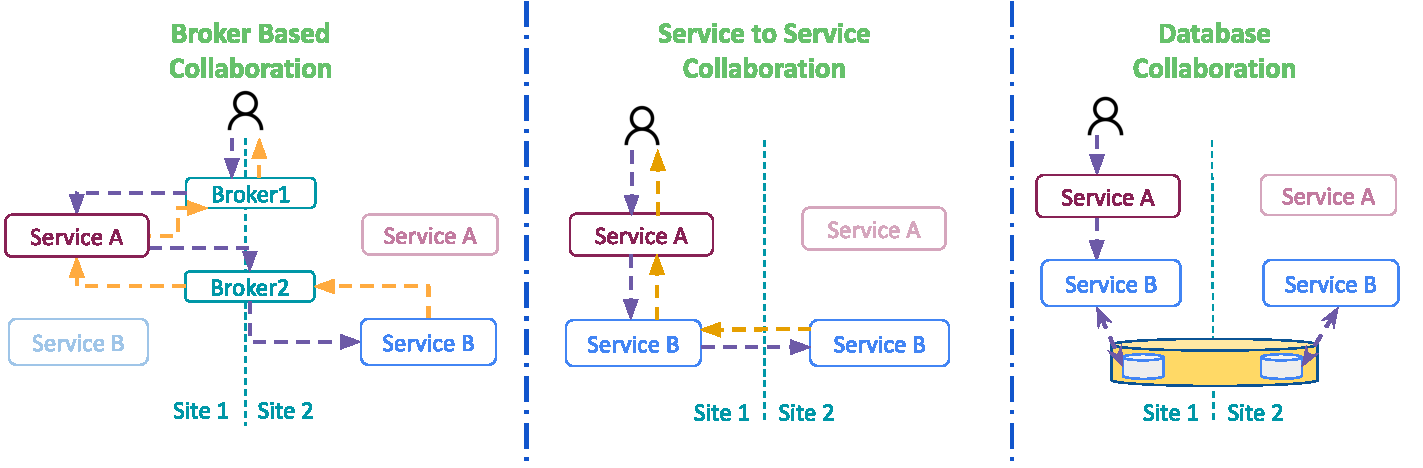
\includegraphics[width=1\textwidth]{figs/pdf/solutions}
  \caption{Different types of solutions}
  \label{fig:edge-solutions}
\end{figure}

\autoref{fig:edge-solutions} presents these three approaches.
%
The first is a broker based solution, which allows for inter-service
collaborations.
%
The broker approach allows externalization of collaboration aspects
away from the business code.
%
However, this approach requires a lot of development effort for an
application.
%
In addition to requiring a broker stub for each service, each broker
should implement once again a lot of what the original functionalities
of the service (because the broker needs to offer the same
capabilities as the underlying service in a geo-distributed and
transparent manner).
%
The alternative is having a generic broker to all services and
applications, which is difficult to envision because of the
differences between them.

Another interesting approach is service-to-service collaborations,
which is an intra-service collaboration.
%
As discussed before, this type of collaboration requires dedicated
code in the service, which is not related to its core logic.

Finally, the third approach is the one we explored previously to this
PhD~\cite{LPSD17, Che17, DCL18}, using databases or data stores, as
the current accepted research direction for developing geo-distributed
applications consists in using globally distributed data
stores~\cite{Aba12}.
%
Distributed data stores emulate a shared memory space among the
different instances of the application to make the development of
geo-distributed application easier~\cite{SBPB+18}.

%
I will now present more thoroughly this approach, as we discovered by
using it why the inherent problems to adopt it for an existing Cloud
application.

%One of the ways to allow


% \autoref{fig:edge-solutions} presents different solutions that are
% available to bring Cloud-native applications to the Edge.



\subsection{In particular: the issue of geo-distributing \os with a distributed data store}
\label{ssec:issue-db}


Most of this part comes from our Euro-Par paper~\cite{CDL21}, and is
also discussed in our Research Report from 2020~\cite{CDLR+20}, both
written with Ronan-Alexandre Cherrueau and Adrien Lebre, and the
second also with Javier Rojas Balderrama and Matthieu Simonin.
%
To explain the issues with this approach, I will use \os as an
example, since it is by trying to use it at this Edge we identified
these issues, and previous studies based on a shared database already
paved the way for \os~\cite{LPSD17, BPC16}.
%
OpenStack is a resource management application to operate one DC.  It
is responsible for booting Virtual Machines (VMs), assigning VMs in
networks, storing operating system images, administrating users, or
any operation related to the management of a DC.
%
It is thus both an Cloud application and an application to manage
Clouds.
%
It is a good example of what we want to geo-distribute, as \os is
around 13M lines of code~\cite{openstackloc}, so a huge application we
do not want to change.


\subsubsection{A complex but modular application.}

Similarly to other Cloud applications, \os follows a modular design
with many services.
%
It has been developed to run natively on one single \gls{dc}.
%
Some efforts have been made along its development to make it run on
multiple clusters, even at large scale.
%
For example, some involved to allow service-to-service collaboration
for specific services (like Keystone~\cite{keystonefed},
Glance~\cite{glance-edge}), but it requires a lot of efforts for all
services to add the features and to maintain them.
%
The compute service for example manages the compute resources of a
\acrshort{DC} to boot VMs.
%
The image service controls operating system \acrshort{blob}s like Debian.
\autoref{fig:os} depicts this modular design in the context of a boot
of a VM.
%
The user starts by addressing a boot request to the compute
service of the DC (Step 1).
%
\begin{figure}[h]
  \centering
  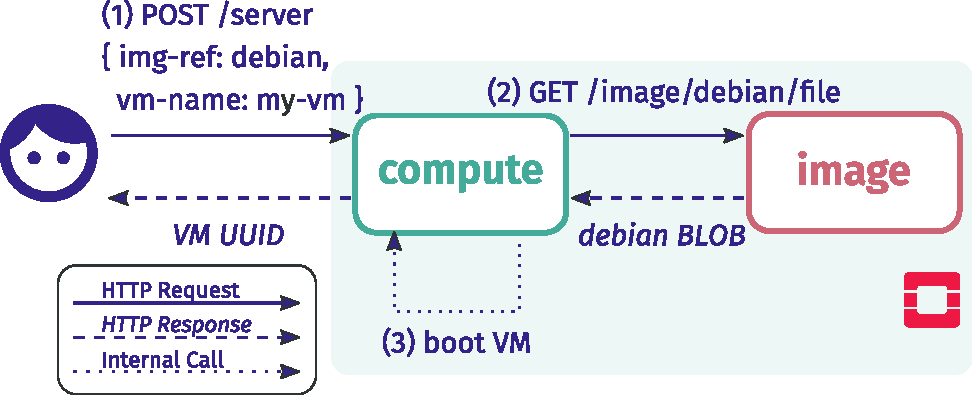
\includegraphics[width=.7\linewidth]{figs/pdf/openstack-vmprovision}
  \caption{Boot of a Debian VM in OpenStack}
  \label{fig:os}
\end{figure}
%
The compute service handles the request and contacts the image service
to get the Debian blob in return (Step 2).
%
Finally, the compute does a bunch of internal calls, such as schedule
VM, setup the network, mount the drive with the blob, before booting
the new VM onto one of its compute nodes (Step 3)\footnote{For
clarity, the boot workflow is simplified here. In a real OpenStack
deployment, the boot also requires at least the network and identity
service. Many other service may also be involved.  See
\url{https://www.openstack.org/software/}.  Accessed 2022-10-02}


\subsubsection{Geo-distributing Openstack.}

Following the local-first and collaborative-then principles implies
two important considerations for OpenStack.
%
First, each DC should behave like a usual cloud infrastructure where
users can make requests and use resources belonging to one site
without any external communication to other sites.
%
Second, users should be able to manipulate resources between DCs if
needed~\cite{CLPW+18}.
%
For instance, \autoref{fig:os-share} illustrates an hypothetical
sharing with the ``boot of a VM at one DC using the Debian image
available in a second one'' scenario.
%
\begin{figure}[h]
  \centering
  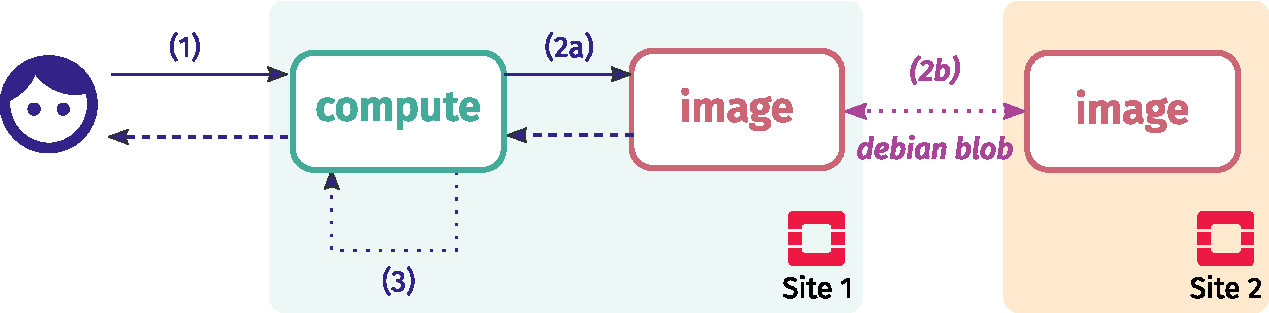
\includegraphics[width=.8\linewidth]{figs/pdf/openstack-share}
  \caption{Boot of a VM using a remote blob}
  \label{fig:os-share}
\end{figure}

To provide this resource sharing between \sOne and \sTwo, the image
service has to implement an additional dedicated means (Step 2b).
%
Moreover, it should be configurable as it might be relevant to
replicate the resource if the sharing is supposed to be done multiple
times over a WAN link.
%
Implementing such a mechanism is a tedious task for programmers of the
application, who might prefer to rely on a distributed data
store~\cite{CDEF+12}.


\subsubsection{Problem: distributed data store tangles the geo-distribution concern.}
\label{ssec:pb1}

The OpenStack image service team studied several solutions to
implement the ``booting a VM at \sOne that benefits from images in
\sTwo'' scenario.
%
All are based on a distributed data store that provides resource
sharing between multiple image services: a pull mode where \sOne
instance gets blobs from \sTwo using a message passing middleware, a
system that replicates blobs around instances using a shared database,
etc.~\cite{glance-edge}
%
The bottom line is that they all require to \emph{entangle} the
geo-distribution concern within the logic of the application.
%
This can be illustrated by the code that retrieves a blob when a
request is issued on the image service (code at Step~2 from
\autoref{fig:os-share}).


\begin{lstlisting}[
    caption={Retrieval of a blob in the image service},
    label=lst:glance,
    numbers=left,
    frame=lines,
    float=tb,
    basicstyle=\footnotesize,
    ]
@app.get('/image/{name}/file')
def get_image(name: String) -> blob:
  # Lookup the image path in the data store:
  # `path = proto://path/debian.qcow`
  path = ds.query(f'''SELECT path FROM images WHERE id IS "{name}";''')

  # Read path to get the image blob
  image_blob = image_collection.get(path)
  return image_blob
\end{lstlisting}

\autoref{lst:glance} gives a coarse-grained description of that code.
%
It first queries the data store to find the path of the blob (l.~5).
%
It then retrieves that blob in the \verb|image_collection| and returns
it to the caller using the \verb|get| method (l.~6--8).
%
Particularly, this method resolves the protocol of the \verb/path/ and
calls the proper library to get the image.
%
Most of the time, that path refers to a blob address on the local disk
(\eg \verb|file:///path/debian.qcow|).
%
In such a case, the method \verb|image_collection.get| relies on the
local \verb|open| python function to get the blob.

\begin{figure}[h]
  \centering
  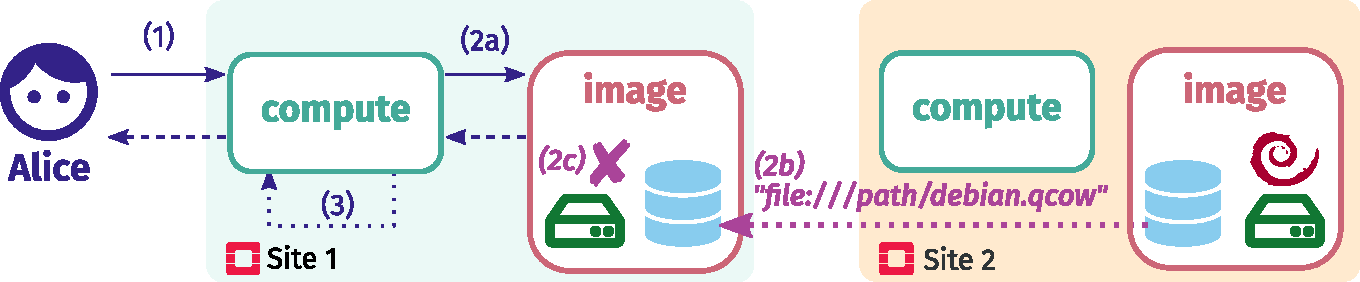
\includegraphics[width=1\linewidth]{figs/pdf/openstack-db-backend}
  \caption{Booting a VM at \sOne with a blob in \sTwo using a
    distributed data store (does not work)}
  \label{fig:glance}
\end{figure}

%
The code executes properly as long as only one OpenStack is involved.
%
But things go wrong when multiple are unified through a data store.
%
\autoref{fig:glance} presents how it is a problem.
%
If \autoref{lst:glance} remains unchanged, then the sole difference in
the workflow of ``booting a VM at \sOne using an image in \sTwo'' is
the distributed data store that federates all image paths (including
those in \sTwo).
%
Unfortunately, because \sTwo hosts the Debian image, the file path of
that image returned at Step 2b is local to \sTwo and \emph{does not
exist} on the disk of \sOne.
%
An \emph{error} results in the \verb|image_collection.get| (2c).

The execution of the method \verb|image_collection.get| takes place in
a specific environment called its \emph{execution context}.
%
This context contains explicit data such as the method parameters.
%
In our case, the image \verb|path| found from the data store.
%
It also contains implicit assumptions made by the programmer: ``A path
with the \verb|file:| prototype must refer to an image stored on the
local disk''.
%
Alas, such kind of assumptions are wrong with a distributed data
store.
%
The code has to be fixed.
%
For this scenario of ``booting a VM at \sOne using an image in
\sTwo'', it means changing the \verb|image_collection.get| method in
order to allow the access of the disk of \sTwo from \sOne.
%
More generally, a distributed data store constrains programmers to
take the distribution into account (and the struggle to achieved it)
in the application.
%
And besides this entanglement, a distributed data store also strongly
limits the collaborative-then principle.
%
In the code above, there is no way to specify whether a particular
blob should be replicated or not, for example.
%

The geo-distribution thus must be handled outside of the business
logic and in a fine-grained manner due to its complexity, along with
the requirements stated before.


\section{Conclusion on the context} % 2p
\label{sec:cccontext}

As we discussed throughout this part (\autoref{p:context}), Cloud
applications were not designed to face the Edge challenges, especially
the disconnections and latency problems inherent to this paradigm.

As we want to bring Cloud appplications to the Edge, and considering
that some are huge, we want to avoid changing their original code as
much as possible and find a generic solution that can be used for a
lot of applications.

This is why I defined these principles for a possible solution:
  \begin{itemize}
  \item \textbf{local-first} to work autonomously
  \item \textbf{collaborative-then} to leverage the infrastructure
  \item \textbf{non-intrusive} regarding the code of the application
  \item \textbf{generic} to a lot of existing applications
  \item \textbf{tolerance to network partition} for the Edge
    disconnections problems
  \item \textbf{dynamic placement} of requests to cope with the
    dynamism of the Edge infrastructure
  \item placement \textbf{decided by the users}, per request, when
    needed
  \item \textbf{decentralized} to avoid single points of failure
    complications
  \item \textbf{P2P} to match the aforementioned principles:
    local-first, tolerance to network partitions, decentralized
  \end{itemize}

  As I was defining the principles required for the solution I want to
  answer my research question of bringing Cloud applications to the
  Edge, I specified the logic of a solution for the collaborations
  between different instances of the exact same application deployed
  on each location while keeping a single coherent system.

  We have overviewed why different solutions for collaborations,
  namely \emph{non-generic brokers},
  \emph{service-to-service}/federation, and \emph{distributed
    databases}, are not generic and imply to code the collaborations
  for each service (broker, service-to-service), or entangle
  non-business information into the code (database), which
  automatically goes against the non-intrusive principle.

  In the next part (\autoref{p:soa}), we will observe how the
  state-of-the-art solutions envision their own different ways to
  bring Cloud applications to the Edge, as well as taking a peek on
  how Edge applications can be developed to check if we can learn
  ideas on how to build this bridge between the two computing
  paradigms.
